\documentclass[twoside]{book}

% Packages required by doxygen
\usepackage{fixltx2e}
\usepackage{calc}
\usepackage{doxygen}
\usepackage[export]{adjustbox} % also loads graphicx
\usepackage{graphicx}
\usepackage[utf8]{inputenc}
\usepackage{makeidx}
\usepackage{multicol}
\usepackage{multirow}
\PassOptionsToPackage{warn}{textcomp}
\usepackage{textcomp}
\usepackage[nointegrals]{wasysym}
\usepackage[table]{xcolor}

% Font selection
\usepackage[T1]{fontenc}
\usepackage[scaled=.90]{helvet}
\usepackage{courier}
\usepackage{amssymb}
\usepackage{sectsty}
\renewcommand{\familydefault}{\sfdefault}
\allsectionsfont{%
  \fontseries{bc}\selectfont%
  \color{darkgray}%
}
\renewcommand{\DoxyLabelFont}{%
  \fontseries{bc}\selectfont%
  \color{darkgray}%
}
\newcommand{\+}{\discretionary{\mbox{\scriptsize$\hookleftarrow$}}{}{}}

% Page & text layout
\usepackage{geometry}
\geometry{%
  a4paper,%
  top=2.5cm,%
  bottom=2.5cm,%
  left=2.5cm,%
  right=2.5cm%
}
\tolerance=750
\hfuzz=15pt
\hbadness=750
\setlength{\emergencystretch}{15pt}
\setlength{\parindent}{0cm}
\setlength{\parskip}{3ex plus 2ex minus 2ex}
\makeatletter
\renewcommand{\paragraph}{%
  \@startsection{paragraph}{4}{0ex}{-1.0ex}{1.0ex}{%
    \normalfont\normalsize\bfseries\SS@parafont%
  }%
}
\renewcommand{\subparagraph}{%
  \@startsection{subparagraph}{5}{0ex}{-1.0ex}{1.0ex}{%
    \normalfont\normalsize\bfseries\SS@subparafont%
  }%
}
\makeatother

% Headers & footers
\usepackage{fancyhdr}
\pagestyle{fancyplain}
\fancyhead[LE]{\fancyplain{}{\bfseries\thepage}}
\fancyhead[CE]{\fancyplain{}{}}
\fancyhead[RE]{\fancyplain{}{\bfseries\leftmark}}
\fancyhead[LO]{\fancyplain{}{\bfseries\rightmark}}
\fancyhead[CO]{\fancyplain{}{}}
\fancyhead[RO]{\fancyplain{}{\bfseries\thepage}}
\fancyfoot[LE]{\fancyplain{}{}}
\fancyfoot[CE]{\fancyplain{}{}}
\fancyfoot[RE]{\fancyplain{}{\bfseries\scriptsize Generated by Doxygen }}
\fancyfoot[LO]{\fancyplain{}{\bfseries\scriptsize Generated by Doxygen }}
\fancyfoot[CO]{\fancyplain{}{}}
\fancyfoot[RO]{\fancyplain{}{}}
\renewcommand{\footrulewidth}{0.4pt}
\renewcommand{\chaptermark}[1]{%
  \markboth{#1}{}%
}
\renewcommand{\sectionmark}[1]{%
  \markright{\thesection\ #1}%
}

% Indices & bibliography
\usepackage{natbib}
\usepackage[titles]{tocloft}
\setcounter{tocdepth}{3}
\setcounter{secnumdepth}{5}
\makeindex

% Hyperlinks (required, but should be loaded last)
\usepackage{ifpdf}
\ifpdf
  \usepackage[pdftex,pagebackref=true]{hyperref}
\else
  \usepackage[ps2pdf,pagebackref=true]{hyperref}
\fi
\hypersetup{%
  colorlinks=true,%
  linkcolor=blue,%
  citecolor=blue,%
  unicode%
}

% Custom commands
\newcommand{\clearemptydoublepage}{%
  \newpage{\pagestyle{empty}\cleardoublepage}%
}

\usepackage{caption}
\captionsetup{labelsep=space,justification=centering,font={bf},singlelinecheck=off,skip=4pt,position=top}

%===== C O N T E N T S =====

\begin{document}

% Titlepage & ToC
\hypersetup{pageanchor=false,
             bookmarksnumbered=true,
             pdfencoding=unicode
            }
\pagenumbering{alph}
\begin{titlepage}
\vspace*{7cm}
\begin{center}%
{\Large My Project }\\
\vspace*{1cm}
{\large Generated by Doxygen 1.8.13}\\
\end{center}
\end{titlepage}
\clearemptydoublepage
\pagenumbering{roman}
\tableofcontents
\clearemptydoublepage
\pagenumbering{arabic}
\hypersetup{pageanchor=true}

%--- Begin generated contents ---
\chapter{File Index}
\section{File List}
Here is a list of all documented files with brief descriptions\+:\begin{DoxyCompactList}
\item\contentsline{section}{\hyperlink{prob1_8c}{prob1.\+c} \\*Determine class, Network and Host ID of an I\+Pv4 address }{\pageref{prob1_8c}}{}
\item\contentsline{section}{\hyperlink{prob2__client_8c}{prob2\+\_\+client.\+c} \\*Client side code for U\+DP socket programming }{\pageref{prob2__client_8c}}{}
\item\contentsline{section}{\hyperlink{prob2__server_8c}{prob2\+\_\+server.\+c} \\*Server side code for U\+DP socket programming }{\pageref{prob2__server_8c}}{}
\item\contentsline{section}{\hyperlink{prob3_8tcl}{prob3.\+tcl} }{\pageref{prob3_8tcl}}{}
\item\contentsline{section}{\hyperlink{prob4_8tcl}{prob4.\+tcl} }{\pageref{prob4_8tcl}}{}
\item\contentsline{section}{\hyperlink{prob5_8tcl}{prob5.\+tcl} }{\pageref{prob5_8tcl}}{}
\end{DoxyCompactList}

\chapter{File Documentation}
\hypertarget{prob1_8cpp}{}\section{prob1.\+cpp File Reference}
\label{prob1_8cpp}\index{prob1.\+cpp@{prob1.\+cpp}}


Problem Statement 1 \+: Prints process\+\_\+ids of created child and grandchild processes.  


{\ttfamily \#include $<$stdio.\+h$>$}\newline
{\ttfamily \#include $<$unistd.\+h$>$}\newline
Include dependency graph for prob1.\+cpp\+:\nopagebreak
\begin{figure}[H]
\begin{center}
\leavevmode
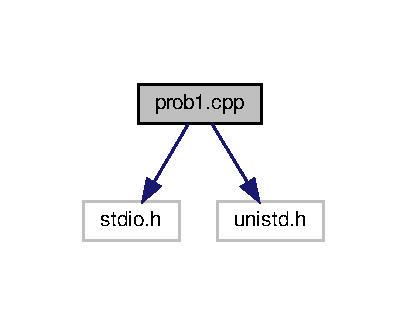
\includegraphics[width=196pt]{prob1_8cpp__incl}
\end{center}
\end{figure}
\subsection*{Functions}
\begin{DoxyCompactItemize}
\item 
\mbox{\Hypertarget{prob1_8cpp_ae66f6b31b5ad750f1fe042a706a4e3d4}\label{prob1_8cpp_ae66f6b31b5ad750f1fe042a706a4e3d4}} 
int {\bfseries main} ()
\end{DoxyCompactItemize}


\subsection{Detailed Description}
Problem Statement 1 \+: Prints process\+\_\+ids of created child and grandchild processes. 

\begin{DoxyAuthor}{Author}
Ayush Agarwal, 17114017 
\end{DoxyAuthor}
\begin{DoxyDate}{Date}
July 2019 
\end{DoxyDate}

\hypertarget{prob2_8cpp}{}\section{prob2.\+cpp File Reference}
\label{prob2_8cpp}\index{prob2.\+cpp@{prob2.\+cpp}}


Problem Statement 2 \+: Demonstrate both Zombie and Orphan process.  


{\ttfamily \#include $<$bits/stdc++.\+h$>$}\newline
{\ttfamily \#include $<$unistd.\+h$>$}\newline
{\ttfamily \#include $<$stdio.\+h$>$}\newline
{\ttfamily \#include $<$sys/wait.\+h$>$}\newline
Include dependency graph for prob2.\+cpp\+:\nopagebreak
\begin{figure}[H]
\begin{center}
\leavevmode
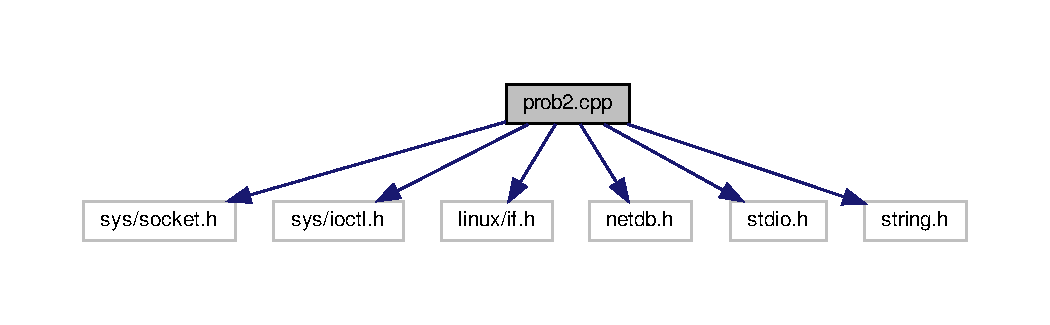
\includegraphics[width=350pt]{prob2_8cpp__incl}
\end{center}
\end{figure}
\subsection*{Functions}
\begin{DoxyCompactItemize}
\item 
\mbox{\Hypertarget{prob2_8cpp_ae66f6b31b5ad750f1fe042a706a4e3d4}\label{prob2_8cpp_ae66f6b31b5ad750f1fe042a706a4e3d4}} 
int {\bfseries main} ()
\end{DoxyCompactItemize}


\subsection{Detailed Description}
Problem Statement 2 \+: Demonstrate both Zombie and Orphan process. 

\begin{DoxyAuthor}{Author}
Ayush Agarwal, 17114017 
\end{DoxyAuthor}
\begin{DoxyDate}{Date}
July 2019 
\end{DoxyDate}

\hypertarget{prob3_8cpp}{}\section{prob3.\+cpp File Reference}
\label{prob3_8cpp}\index{prob3.\+cpp@{prob3.\+cpp}}


Problem Statement 3 \+: Ping a server.  


{\ttfamily \#include $<$stdio.\+h$>$}\newline
{\ttfamily \#include $<$stdlib.\+h$>$}\newline
{\ttfamily \#include $<$arpa/inet.\+h$>$}\newline
{\ttfamily \#include $<$sys/socket.\+h$>$}\newline
{\ttfamily \#include $<$fcntl.\+h$>$}\newline
{\ttfamily \#include $<$unistd.\+h$>$}\newline
{\ttfamily \#include $<$netdb.\+h$>$}\newline
{\ttfamily \#include $<$string.\+h$>$}\newline
Include dependency graph for prob3.\+cpp\+:\nopagebreak
\begin{figure}[H]
\begin{center}
\leavevmode
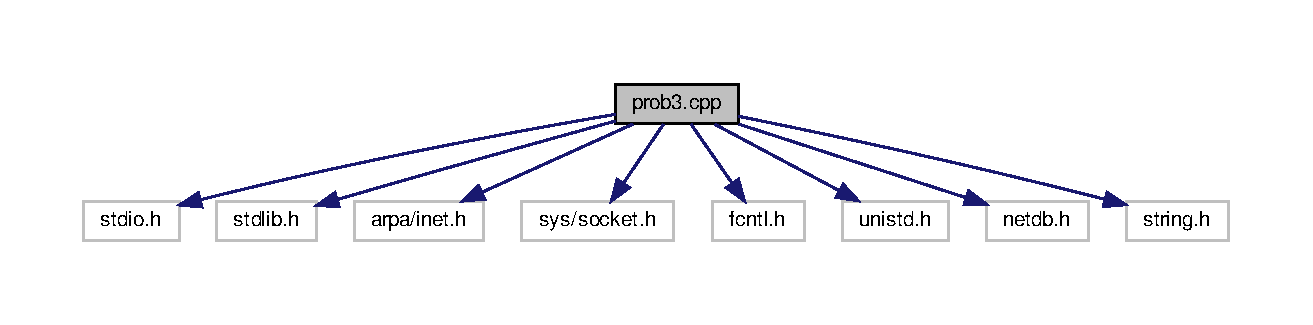
\includegraphics[width=350pt]{prob3_8cpp__incl}
\end{center}
\end{figure}
\subsection*{Functions}
\begin{DoxyCompactItemize}
\item 
\mbox{\Hypertarget{prob3_8cpp_a37b251fb907c1eee05fd01b71be56cb2}\label{prob3_8cpp_a37b251fb907c1eee05fd01b71be56cb2}} 
char $\ast$ {\bfseries dns\+\_\+lookup} (char $\ast$addr\+\_\+host, struct sockaddr\+\_\+in $\ast$addr\+\_\+con)
\item 
\mbox{\Hypertarget{prob3_8cpp_a0ddf1224851353fc92bfbff6f499fa97}\label{prob3_8cpp_a0ddf1224851353fc92bfbff6f499fa97}} 
int {\bfseries main} (int argc, char $\ast$argv\mbox{[}$\,$\mbox{]})
\end{DoxyCompactItemize}


\subsection{Detailed Description}
Problem Statement 3 \+: Ping a server. 

\begin{DoxyAuthor}{Author}
Ayush Agarwal, 17114017 
\end{DoxyAuthor}
\begin{DoxyDate}{Date}
July 2019 
\end{DoxyDate}

\hypertarget{prob4_8cpp}{}\section{prob4.\+cpp File Reference}
\label{prob4_8cpp}\index{prob4.\+cpp@{prob4.\+cpp}}


Problem Statement 4 \+: Get the host name and the IP address of your computer.  


{\ttfamily \#include $<$stdio.\+h$>$}\newline
{\ttfamily \#include $<$stdlib.\+h$>$}\newline
{\ttfamily \#include $<$unistd.\+h$>$}\newline
{\ttfamily \#include $<$errno.\+h$>$}\newline
{\ttfamily \#include $<$netdb.\+h$>$}\newline
{\ttfamily \#include $<$sys/types.\+h$>$}\newline
{\ttfamily \#include $<$sys/socket.\+h$>$}\newline
{\ttfamily \#include $<$netinet/in.\+h$>$}\newline
{\ttfamily \#include $<$arpa/inet.\+h$>$}\newline
Include dependency graph for prob4.\+cpp\+:\nopagebreak
\begin{figure}[H]
\begin{center}
\leavevmode
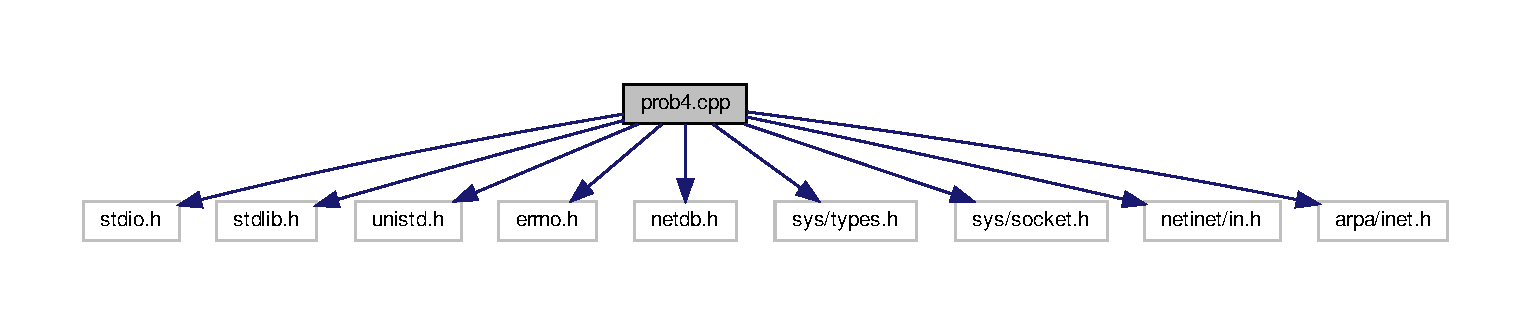
\includegraphics[width=350pt]{prob4_8cpp__incl}
\end{center}
\end{figure}
\subsection*{Functions}
\begin{DoxyCompactItemize}
\item 
\mbox{\Hypertarget{prob4_8cpp_ae66f6b31b5ad750f1fe042a706a4e3d4}\label{prob4_8cpp_ae66f6b31b5ad750f1fe042a706a4e3d4}} 
int {\bfseries main} ()
\end{DoxyCompactItemize}


\subsection{Detailed Description}
Problem Statement 4 \+: Get the host name and the IP address of your computer. 

\begin{DoxyAuthor}{Author}
Ayush Agarwal, 17114017 
\end{DoxyAuthor}
\begin{DoxyDate}{Date}
July 2019 
\end{DoxyDate}

%--- End generated contents ---

% Index
\backmatter
\newpage
\phantomsection
\clearemptydoublepage
\addcontentsline{toc}{chapter}{Index}
\printindex

\end{document}
